\documentclass[]{article}
\usepackage{proceed2e}
\usepackage{amssymb,amsmath,amsthm}
\usepackage{graphicx}
\usepackage{preamble}
\usepackage{natbib}
\usepackage{hyperref}
\usepackage{color}
\definecolor{mydarkblue}{rgb}{0,0.08,0.45}
\hypersetup{ %
    pdftitle={},
    pdfauthor={},
    pdfsubject={},
    pdfkeywords={},
    pdfborder=0 0 0,
    pdfpagemode=UseNone,
    colorlinks=true,
    linkcolor=mydarkblue,
    citecolor=mydarkblue,
    filecolor=mydarkblue,
    urlcolor=mydarkblue,
    pdfview=FitH}



\title{Bayesian Quadrature minimizes Maximum Mean Discrepancy}

\author{ {\bf Ferenc Husz\'{a}r} \\
Department of Engineering\\
Cambridge University\\ 
\texttt{fh277@cam.ac.uk}
\And 
{\bf David Duvenaud } \\ %\thanks{Both authors contributed equally.} \\ 
Department of Engineering\\ 
Cambridge University \\
\texttt{dkd23@cam.ac.uk}
} 

\begin{document} 
 
\maketitle 
 
%\begin{abstract} 
%Maximum Mean Discrepancy is equivalent to the posterior variance of an integrated Gaussian process.
%\end{abstract} 

 
\section{INTRODUCTION}
A common problem in statistical machine learning is to compute expectations of functions over probability distributions of the form:
\begin{equation}
	Z_{f,p} = \int f(x) p(x) dx \label{eqn:integral}
\end{equation}
Examples include computing marginal distributions, making predictions marginalizing over parameters, or computing the Bayes risk in a decision problem. %In this paper we assume that the distribution $p(x)$ is known in analytic form, and $f(x)$ can be evaluated at arbitrary locations.

%Monte Carlo methods produce random samples from the distribution $p$ and then approximate the integral by taking the empirical mean $\hat{Z} = \frac{1}{N}\sum_{n=1}^{N}f_{x_n}$ of the function evaluated at those points. This non-deterministic estimate converges at a rate $\mathcal{O}(\frac{1}{\sqrt{N}})$. When exact sampling from $p$ is impossible or impractical, Markov chain Monte Carlo (MCMC) methods are often used. MCMC methods can be applied to almost any problem but convergence of the estimate depends on several factors and is hard to estimate \citep{CowlesCarlin96}. The focus of this paper is on quasi-Monte Carlo methods that -- instead of sampling randomly -- produce a set of pseudo-samples in a deterministic fashion. These methods operate by directly minimising some sort of discrepancy between the empirical distribution of pseudo-samples and the target distribution. Whenever these methods are applicable, they achieve convergence rates superior to the $\mathcal{O}(\frac{1}{\sqrt{N}})$ rate typical of random sampling.

%In this paper we highlight and explore the connections between two deterministic sampling and integration methods: Bayesian quadrature (\bq{}) \citep{BZHermiteQuadrature,BZMonteCarlo} (also known as Bayesian Monte Carlo) and kernel herding \citep{chen2010super}. Bayesian quadrature estimates integral \eqref{eqn:integral} by inferring a posterior distribution over $f$ conditioned on the observed evaluations $f_{x_n}$, and then computing the posterior expectation of $Z_{f,p}$. The points where the function should be evaluated can be found via Bayesian experimental design, providing a deterministic procedure for selecting sample locations.% We call this procedure Sequential Bayesian Quadrature (\sbq).

%Herding, proposed recently by \cite{chen2010super}, produces pseudosamples by minimising the discrepancy of moments between the sample set and the target distribution. Similarly to traditional Monte Carlo, an estimate is formed by taking the empirical mean over samples $\hat{Z} = \frac{1}{N}\sum_{n=1}^{N}f_{x_n}$. Under certain assumptions, herding has provably fast, $\mathcal{O}(\frac{1}{N})$ convergence rates in the parametric case, and has demonstrated strong empirical performance in a variety of tasks.

In this paper, we make two main contributions.  Firs, we show that the Maximum Mean Discrepancy (MMD) criterion (used to choose samples in kernel herding) is identical to the expected error in the estimate of the integral $Z_{f,p}$ under a Gaussian process prior for $f$.  This expected error is the criterion being minimized when choosing samples for Bayesian quadrature (BQ).  Because Bayesian quadrature assigns different weights to each of the observed function values $f(\vx)$, we can view Bayesian quadrature as a weighted version of kernel herding.  
 We show that these weights are optimal in a minimax sense over all functions in the Hilbert space defined by our kernel.  This implies that Bayesian quadrature dominates kernel herding and other non-optimally weighted herding in rate of convergence.

We further show that the MMD, when using BQ weights, is submodular in the samples chosen, which implies that sequential BQ achieves the optimal rate of convergence for any sampling method.

\section{HERDING} 

Herding was introduced by \cite{welling2009herding} as a method for generating pseudo-samples from a distribution in such a way that certain nonlinear moments of the sample set closely match those of the target distribution.  The empirical mean $\frac{1}{N}\sum_{n=1}^{N}f_{x_n}$ over these pseudosamples is then used to estimate integral \eqref{eqn:integral}.

\subsection{Maximum Mean Discrepancy}

For selecting pseudosamples, herding relies on an objective based on the maximum mean discrepancy \citep[MMD;\ ][]{Sriperumbudur2010}: %MMD measures the divergence between two distributions, $p$ and $q$ with respect to a class of integrand functions $\mathcal{F}$ as follows:
%
\begin{align}
	\mmd_{\mathcal{F}}\left(p,q\right) = \sup_{f\in\mathcal{F}}\left\vert\int f_x p(x) dx - \int f_x q(x) dx \right\vert
\end{align}
%
%Intuitively, if two distributions are close in the MMD sense, then no matter which function $f$ we choose from $\mathcal{F}$, the difference in its integral over $p$ or $q$ should be small. A particularly interesting case is 
%
When the function class $\mathcal{F}$ is functions of unit norm from a reproducing kernel Hilbert space (RKHS) $\He$, the MMD between two distributions can be conveniently expressed using only expectations of the associated kernel $k(x, x')$ \citep{Sriperumbudur2010}.
%
%\begin{align}
%MMD^2_{\He}(p,q) =& \sup_{\substack{f\in\He\\\Hnorm{f}=1}}\left\vert\int f_x p(x) dx - \int f_x q(x) dx\right\vert^2\\
%	=& \Hnorm{\mu_{p} - \mu_{q}}^2\\
%\nonumber	=&\iint k(x,y) p(x) p(y) dx dy\\
%\nonumber	-2 &\iint k(x,y) p(x) q(y) dx dy\\
%	+ &\iint k(x,y) q(x) q(y) dx dy,
%\end{align}
%
%where in the above formula $\mu_{p}=\int \phi(\vx)p(\vx)d\vx\in\He$ denotes the \emph{mean element} associated with the distribution $p$.
% For characteristic kernels, such as the Gaussian kernel, the mapping between a distribution and its mean element is bijective. As a consequence $\mmd_{\He}(p,q)=0$ if and only if $p=q$, making it a powerful measure of divergence.
%
Herding uses MMD to evaluate how well the sample set $\{\vx_1,\ldots,\vx_{N}\}$ represents the target distribution $p$, adding points greedily according to:
%
%\begin{align}
%	\epsilon_{herding}&\left(\{\vx_1,\ldots,\vx_{N}\}\right) = \mmd_{\He}\left(p,\frac{1}{N}\sum_{n=1}^{N}\delta_{x_n}\right)\\
%\nonumber	=&\iint k(x,y) p(x) p(y) dx dy\\
%		-2 &\frac{1}{N}\sum_{n=1}^{N}\int k(x,x_n) p(x) dx
%		+ \frac{1}{N^2}\sum_{n,m=1}^{N} k(x_n,x_m)
%\label{eq:mmd_assumption}
%\end{align}
%
%The herding procedure greedily minimizes its objective $\epsilon_{herding}\left(\{\vx_1,\ldots,\vx_{N}\}\right)$ , adding pseudosamples $\vx_n$ one at a time. When selecting the $n+1$-st pseudosample:
%
\begin{align}
\vx_{n+1} &\leftarrow \argmin_{\vx \in \mathcal{X}} \label{eqn:herding_criterion} \epsilon_{herding}\left(\{\vx_1,\ldots,\vx_{n},\vx\}\right)\\
	&= \argmax_{\vx \in \mathcal{X}} 2 \expectargs{\vx' \sim p}{k(\vx, \vx')} - \frac{1}{n+1}\sum_{m=1}^{n} k(\vx,\vx_m)\mbox{,}\notag
\end{align}
%
assuming $k(\vx,\vx) = \mbox{const}$.
The formula \eqref{eqn:herding_criterion} admits an intuitive interpretation: the first term encourages sampling in areas with high mass under the target distribution $p(\vx)$.  The second term discourages sampling at points close to existing samples. 




\section{BAYESIAN QUADRATURE} 

%\begin{figure}
%\centering
%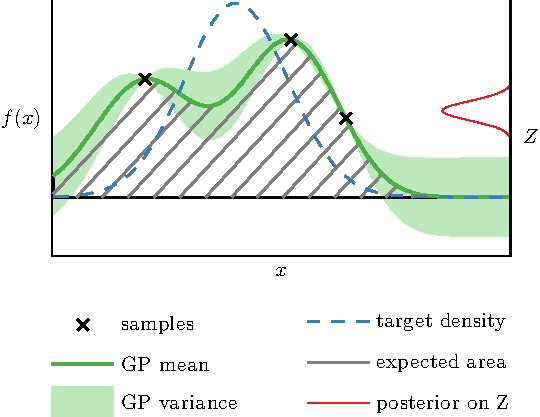
\includegraphics[width=\columnwidth]{figures/bq_intro4}
%\caption{An illustration of Bayesian Quadrature.  The function $f(x)$ is sampled at a set of input locations.  %This induces a Gaussian process posterior distribution on $f$, which is integrated in closed form against the target density, $p(\vx)$.  Since the amount of volume under $f$ is uncertain, this gives rise to a (Gaussian) posterior distribution over $Z_{f,p}$.}
%\label{fig:bq_intro}
%\end{figure}

Bayesian quadrature (\bq) puts a prior distribution on $\vf$, then estimates integral \eqref{eqn:integral} by inferring a posterior distribution over the function $\vf$, conditioned on the observations $\vf(\vx_n)$ at some query points $\vx_n$.  For simplicity, $\vf$ is assigned a Gaussian process prior with kernel function $k$ and mean $0$.  This assumption is very similar to the one made by kernel herding.  The posterior distribution over $f$ then implies a distribution over $Z_{f,p}$. %See Figure \ref{fig:bq_intro} for an illustration of Bayesian Quadrature.
%
%\subsection{ BQ Estimator}
%
%Here we derive the \bq{} estimate of \eqref{eqn:integral}, after conditioning on function evaluations $\vf(\vx_1) \dots \vf(\vx_N)$, denoted as $f(\vX)$.  
 The mean of this distribution, $\expectargs{}{Z}$ is the optimal Bayesian estimator for a squared loss.
%After conditioning on $\vf(\vX)$, we obtain a closed-form posterior over $\vf$.
%
%\begin{align}
%p(\vf(\vx\st)|\vf(\vX)) = \N{\vf(\vx\st)}{\mf(\vx\st)}{\cov(\vx\st,\vx\st')}
%\end{align} 
%where
%\begin{align}
%\mf(\vx\st) = & k(\vx\st, \vX) K^{-1} \vf(\vX) \\
%\cov(\vx\st, \vx\st') = & k(\vx\st,\vx\st) - k(\vx\st, \vX) K^{-1} k(\vX, \vx\st)
%\end{align} 
%
%and $K = k(\vX, \vX)$. 
%
Conveniently, the \gp{} posterior allows us to compute the expectation of \eqref{eqn:integral} in closed form: 
%
%\begin{align}
%Z & = \int f(\vx)p(\vx)d\vx
%\end{align} 
%so we integrate over functions to get:
\begin{align}
\expectargs{\gp}{Z} & = \vz^T K^{-1} \vf(\vX)
\label{eq:marg_mean_symbolic}
\end{align} 
where
\begin{align}
z_n & = \int\!\! k(\vx, \vx_n) p(\vx) d\vx = \expectargs{\vx' \sim p}{k(\vx_n, \vx')}.
\end{align}
%
As in kernel herding, the desired expectation of $Z_{f,p}$ is simply a linear combination of observed function values $\vf(\vx)$:
%
\begin{align}
\expectargs{\gp}{Z} & = \vz^T K^{-1} \vf(\vX) \\
    & = \sum_n w_{\bq}^{(n)} f(x_n)  \quad \textrm{where} \quad w_{\bq}^{(n)} = \sum_m \vz_j K^{-1}_{nm}
\end{align}  
%
%\begin{align}  
%w_{\bq}^{(n)} & = \sum_m \vz_j K^{-1}_{nm}
%\label{eq:bq_weights}
%\end{align}
%
Thus, we can view the BQ estimate as a weighted version of the herding estimate.


\subsection{Optimal sampling for BQ}

The posterior variance $\varianceargs{}{Z_{f,p}|f_{x_1}, \dots, f_{x_N}}$ quantifies our uncertainty in the estimate of the integral. When selecting locations to evaluate the function $f$, minimising the posterior variance is a sensible strategy. Below, we give a closed form formula for the posterior variance of $Z_{f,p}$, conditioned on the observations $f_{x_1} \dots f_{x_N}$, which we will denote by $\epsilon^2_{\bq{}}$.
\begin{align}
\epsilon^{2}_{\bq{}} = \varianceargs{}{Z_{f,p}|f_{x_1}, \dots, f_{x_N}} 
% \nonumber & = \expectargs{f \sim \gp, p\sim p(x)}{ \left( f(\vx) - \mf(\vx) \right)\left( f(\vx') - \mf(\vx') \right)} \\ 
%\nonumber & = \int \Bigg( \!\! \left( \int f(\vx) p(\vx) d\vx - \int \mf(\vx') p(\vx') d\vx' \right) \\ 
%\nonumber & \quad \times \left( \int f(\vx) p(\vx) d\vx - \int \mf(\vx') p(\vx') d\vx' \right) \!\! \Bigg) p(f) df \\ 
%\nonumber & = \int\!\!\! \int\!\! \int\!\! \left[ f(\vx) - \mf(\vx) \right] \left[ f((\vx') - \mf(\vx') \right] p(f) df \\
%\nonumber & \qquad \times   p(\vx) p(\vx') d\vx d\vx' \\
%\nonumber & = \int\!\! \!\int\!\! \Cov \left[ f((\vx), f((\vx') \right] p(\vx) p(\vx') d\vx d\vx' \\
%\nonumber & = \int\!\!\! \int\!\! \left[ k(\vx, \vx') - k(\vx, \vX) K^{-1} k(\vX, \vx') \right] \\
%\nonumber          & \qquad \times p(\vx) p(\vx') d\vx d\vx' \\ 
%\nonumber & = \int\!\!\! \int\!\! k(\vx, \vx') p(\vx) p(\vx') d\vx d\vx' \\
%\nonumber & \quad - \left[ \int\!\! k(\vx, \vX) p(\vx) d\vx \right] K^{-1} \left[ \int\!\! k(\vX, \vx') p(\vx') d\vx' \right] \\
  = \expectargs{\vx, \vx' \sim p}{k(\vx, \vx')} - \vz K^{-1} \vz\mbox{,}
\label{eq:marg_var_symbolic}
\end{align}
%where $\vz_n = \expectargs{\vx' \sim p}{k(\vx_n, \vx')}$ as before. 
Perhaps surprisingly, the posterior variance of $Z_{f,p}$ does not depend on the observed function values, only on the location $x_n$ of samples.  This allows the optimal samples to be computed ahead of time, before observing any values of $f$ at all \citep{minka2000dqr}.
%\begin{align}
%\epsilon^{2}_{\bq{}}(\vx_1,\ldots,\vx_N) = \expectargs{\vx, \vx' \sim p}{k(\vx, \vx')} - \vz K^{-1} \vz
%\end{align}
%We can contrast the \bq{} objective $\epsilon^{2}_{\bq{}}$ to the objective being minimized in herding, $\epsilon^{2}_{herding}$ of equation \eqref{eq:mmd_assumption}. 
%Just like $\epsilon^{2}_{herding}$, $\epsilon^{2}_{\bq{}}$ expresses a trade-off between accuracy and diversity of samples. On the one hand, as samples get close to high density regions under $p$, the values in $\vz$ increase, which results in decreasing variance. On the other hand, as samples get closer to each other, eigenvalues of $K$ increase, resulting in an increase in variance. 

\section{RELATING $\varianceargs{}{Z_{f,p}}$ TO $\mmd$}

The similarity in the behaviour of $\epsilon^{2}_{herding}$ and $\epsilon^{2}_{\bq{}}$ is not a coincidence, the two quantities are closely related to each other, and to \mmd.

\begin{prop} The expected variance in the Bayesian quadrature $\epsilon^{2}_{\bq{}}$  is the maximum mean discrepancy between the target distribution $p$ and $q_{\bq{}}(x) = \sum_{n=1}^{N}w^{(n)}_{\bq{}}\delta_{x_n}(x)$
\end{prop}
%
%\begin{proof} Proof omitted for space reasons.
%The proof involves invoking the representer theorem, using bilinearity of scalar products and the fact that if $f$ is a standard Gaussian process then $\forall g\in\He: \left\langle f,g\right\rangle \sim \mathcal{N}(0,\Hnorm{g})$:
%\begin{align}
%&\varianceargs{}{Z_{f,p}\vert f_{x_1}, \dots, f_{x_N}}=\\
%	&= \mathbb{E}_{f\sim GP} \left( \int f(x) p(x) dx - \sum_{n=1}^{N}w^{(n)}_{\bq{}} f(x_n)\right)^2\\
%	&= \mathbb{E}_{f\sim GP} \left( \int \left\langle f, \phi (x)\right\rangle p(x) dx - \sum_{n=1}^{N}w^{(n)}_{\bq{}} \left\langle f, \phi (x_n)\right\rangle\right)^2\\
%	&= \mathbb{E}_{f\sim GP} \left\langle f ,  \int\phi(x) dx - \sum_{n=1}^{N}w^{(n)}_{\bq{}}\phi(x_n)\right\rangle^2\\
%	&= \Hnorm{\mu_p - \mu_{q_{\bq{}}}}^2\\
%	&= \mmd^2(p,q_{\bq{}})
%\end{align}
%\end{proof}

We know that the the posterior mean $\expectargs{\gp}{Z_{f,p}\vert f_1,\ldots,f_N}$ is a Bayes estimator and has therefore the minimal expected squared error amongst all estimators. This allows us to further rewrite $\epsilon^{2}_{\bq{}}$ into the following minimax forms:
%
\begin{align}
\epsilon^{2}_{\bq{}} %&= \sup_{\substack{f\in\He\\\Hnorm{f}{\He}=1}} \left| \int f_x p(x) dx - \sum_{n=1}^{N}w^{(n)}_{\bq{}} f_{x_n}\right|^2\\
%	&= \inf_{\hat{Z}:\mathcal{X}^N\mapsto\mathbb{R}} \sup_{\substack{f\in\He\\\Hnorm{f}{\He}=1}} \left| Z - \hat{Z}\left(f_{x_1},\ldots,f_{x_N}\right)\right|^2\\
	&= \inf_{\bm{w}\in\mathbb{R}^N} \sup_{\substack{f\in\He\\\Hnorm{f}{\He}=1}} \left| \int f_x p(x) dx - \sum_{n=1}^{N}w_n 	f_{x_n}\right|^2
\end{align}
%
%Looking at $\epsilon^{2}_{\bq{}}$  this way, we may discover the deep similarity to the criterion $\epsilon^2_{herding}$ that kernel herding minimises. 
Optimal sampling for Bayesian quadrature minimises the same objective as kernel herding, but with the uniform $\frac{1}{N}$ weights replaced by the optimal weights. As a corollary
%
\begin{align}
\epsilon^{2}_{\bq{}}(x_1,\ldots,x_N)  \leq \epsilon^{2}_{KH} (x_1,\ldots,x_N)
\end{align}
%
It is interesting that $\epsilon^{2}_{\bq{}}$ has both a Bayesian interpretation as posterior variance under a Gaussian process prior, and a frequentist interpretation as a minimax bound on estimation error with respect to an RKHS.  Figure \ref{fig:bound_curve} demonstrates this closed-form, quickly shrinking bound on the error of the Bayesian estimator.  This equivalence also implies that the MMD is proportional to the expected error when estimating integrals of functions drawn from a GP prior.
\begin{figure}
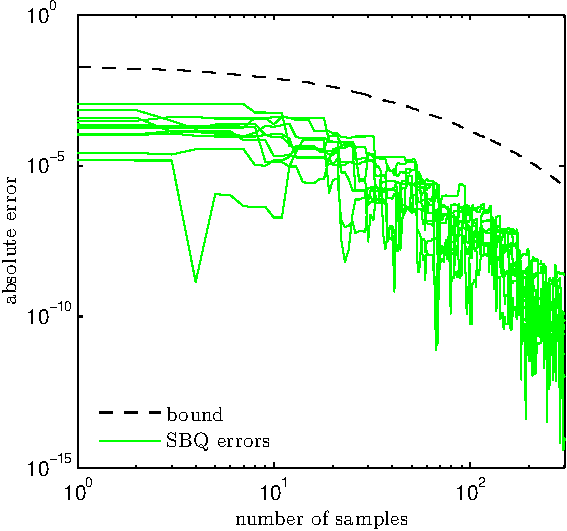
\includegraphics[width=\columnwidth]{figures/bound_curve_rkhs}
\caption{The empirical error rate in estimating $Z_{f,p}$,  for the \sbq{} estimator, on 10 random functions drawn from the RKHS corresponding to the kernel used.  Also shown is the upper bound on the error rate implied by the $\mmd$.}
\label{fig:bound_curve}
\end{figure}
%
%Figure \ref{fig:bound_curve} demonstrates the MMD bound on the error of the \sbq{} estimator, on random functions drawn from the RKHS corresponding to the kernel used.  The empirical error always falls below the bound given by the MMD.


\subsection{Convergence Rates}

In finite dimensional Hilbert spaces, the herding algorithm has been shown to reduce $\mmd$ at a rate $\mathcal{O}(\frac{1}{N})$, which compares favourably with the $\mathcal{O}(\frac{1}{\sqrt{N}})$ rate obtained by non-deterministic Monte Carlo samplers.% However, as pointed out by \cite{bach2012equivalence}, this fast convergence is not guaranteed in infinite dimensional Hilbert spaces, such as the RKHS corresponding to the Gaussian kernel.
we have shown that the greedy Bayesian estimator obtains the optimal rate for any sampling method.  We have empirical results demonstrating a rate of convergence much faster than $\mathcal{O}(\frac{1}{N})$, but this rate is unkown to the authors, and we wish to pose this question to the kernel community.

\pagebreak

\bibliographystyle{icml2012}
\bibliography{herding}

\end{document} 
